%%%%%%%%%%%%%%%%%%%%%%%%%%%%%%%%%%%%%%
% LaTeX poster template
% Created by Nathaniel Johnston
% August 2009
% http://www.nathanieljohnston.com/2009/08/latex-poster-template/
%%%%%%%%%%%%%%%%%%%%%%%%%%%%%%%%%%%%%%

\documentclass[handout,final]{beamer}
\usepackage{beamerposter}
\usepackage{graphicx}			% allows us to import images

\usepackage{booktabs}
\usepackage{bm}
\usepackage{tikz}

\usetikzlibrary{trees,shadows}

\tikzset{/tikz/x=2.5cm}
\tikzset{/tikz/y=2.5cm}

\newcommand{\Ptransmission}{P_{\textit{transmission}}}%

%-----------------------------------------------------------
% Define the column width and poster size
% To set effective sepwid, onecolwid and twocolwid values, first choose how many columns you want and how much separation you want between columns
% The separation I chose is 0.024 and I want 4 columns
% Then set onecolwid to be (1-(4+1)*0.024)/4 = 0.22
% Set twocolwid to be 2*onecolwid + sepwid = 0.464
%-----------------------------------------------------------

\newlength{\sepwid}
\newlength{\onecolwid}
\newlength{\twocolwid}
\newlength{\threecolwid}
\setlength{\paperwidth}{48in}
\setlength{\paperheight}{36in}
\setlength{\sepwid}{0.024\paperwidth}
\setlength{\onecolwid}{0.22\paperwidth}
\setlength{\twocolwid}{0.464\paperwidth}
\setlength{\threecolwid}{0.708\paperwidth}
\setlength{\topmargin}{-0.5in}
\usetheme{confposter}
\usepackage{exscale}

% New math commands/abreviations

\newcommand{\bA}{\mathbf{A}}
\newcommand{\bB}{\mathbf{B}}
\newcommand{\bC}{\mathbf{C}}
\newcommand{\bD}{\mathbf{D}}
\newcommand{\bE}{\mathbf{E}}
\newcommand{\bF}{\mathbf{F}}
\newcommand{\bG}{\mathbf{G}}
\newcommand{\bH}{\mathbf{H}}
\newcommand{\bI}{\mathbf{I}}
\newcommand{\bJ}{\mathbf{J}}
\newcommand{\bK}{\mathbf{K}}
\newcommand{\bL}{\mathbf{L}}
\newcommand{\bM}{\mathbf{M}}
\newcommand{\bN}{\mathbf{N}}
\newcommand{\bO}{\mathbf{O}}
\newcommand{\bP}{\mathbf{P}}
\newcommand{\bQ}{\mathbf{Q}}
\newcommand{\bR}{\mathbf{R}}
\newcommand{\bS}{\mathbf{S}}
\newcommand{\bT}{\mathbf{T}}
\newcommand{\bU}{\mathbf{U}}
\newcommand{\bV}{\mathbf{V}}
\newcommand{\bW}{\mathbf{W}}
\newcommand{\bX}{\mathbf{X}}
\newcommand{\bY}{\mathbf{Y}}
\newcommand{\bZ}{\mathbf{Z}}

\newcommand{\ba}{\mathbf{a}}
%\newcommand{\bb}{\mathbf{b}}
\newcommand{\bc}{\mathbf{c}}
\newcommand{\bd}{\mathbf{d}}
\newcommand{\be}{\mathbf{e}}
%\newcommand{\bf}{\mathbf{f}}
\newcommand{\bg}{\mathbf{g}}
\newcommand{\bh}{\mathbf{h}}
\newcommand{\bi}{\mathbf{i}}
\newcommand{\bj}{\mathbf{j}}
\newcommand{\bk}{\mathbf{k}}
\newcommand{\bl}{\mathbf{l}}
%\newcommand{\bm}{\mathbf{m}}
\newcommand{\bn}{\mathbf{n}}
%\newcommand{\bo}{\mathbf{o}}
\newcommand{\bp}{\mathbf{p}}
\newcommand{\bq}{\mathbf{q}}
\newcommand{\br}{\mathbf{r}}
\newcommand{\bs}{\mathbf{s}}
\newcommand{\bt}{\mathbf{t}}
\newcommand{\bu}{\mathbf{u}}
\newcommand{\bv}{\mathbf{v}}
\newcommand{\bw}{\mathbf{w}}
\newcommand{\bx}{\mathbf{x}}
\newcommand{\by}{\mathbf{y}}
\newcommand{\bz}{\mathbf{z}}

\newcommand{\bff}{\mathbf{f}}

\newcommand{\bo}{\mathbf{0}}
\newcommand{\tx}{\tilde{\mathbf{x}}}


\newcommand{\hbn}{{\widehat{\mathbf{n}}}}
\newcommand{\hbs}{{\widehat{\mathbf{s}}}}
\newcommand{\hbh}{{\widehat{\mathbf{h}}}}
\newcommand{\hbv}{{\widehat{\mathbf{v}}}}
\newcommand{\hbw}{{\widehat{\mathbf{w}}}}
\newcommand{\hbc}{{\widehat{\mathbf{c}}}}

\newcommand{\hh}{{\widehat{h}}}
\newcommand{\hn}{{\widehat{n}}}
\newcommand{\hx}{{\widehat{x}}}
\newcommand{\hy}{{\widehat{y}}}
\newcommand{\hz}{{\widehat{z}}}


% Mathcal definitions
\newcommand{\cS}{\mathcal{S}}
\newcommand{\cD}{\mathcal{D}}
\newcommand{\cP}{{\mathcal{P}}}
\newcommand{\cU}{{\mathcal{U}}}
\newcommand{\cV}{{\mathcal{V}}}
\newcommand{\cE}{{\mathcal{E}}}
\newcommand{\cQ}{{\mathcal{Q}}}
\newcommand{\cG}{{\mathcal{G}}}
\newcommand{\cB}{{\mathcal{B}}}
\newcommand{\cI}{\mathcal{I}}
\newcommand{\cL}{\mathcal{L}}
\newcommand{\cR}{{\mathcal{R}}}
\newcommand{\cC}{{\mathcal{C}}}
\newcommand{\cO}{{\mathcal{O}}}
\newcommand{\cX}{{\mathcal{X}}}



% Mathbb definitions
\newcommand{\bbp}{\mathbb{P}}
\newcommand{\bbP}{\mathbb{P}}
\newcommand{\bbQ}{\mathbb{Q}}
\newcommand{\bbr}{\mathbb{R}}
\newcommand{\bbR}{\mathbb{R}}
\newcommand{\bbS}{\mathbb{S}}
\newcommand{\bbN}{\mathbb{N}}



% Mathbm definitions
\newcommand{\balpha}{{\bm{\alpha}}}
\newcommand{\bbeta}{{\bm{\beta}}}
\newcommand{\bgamma}{{\bm{\gamma}}}
\newcommand{\bepsilon}{{\bm{\epsilon}}}
\newcommand{\bmu}{{\bm{\mu}}}
\newcommand{\bpi}{\bm{\pi}}
\newcommand{\brho}{\bm{\rho}}
\newcommand{\bomega}{\bm{\omega}}
\newcommand{\bOmega}{\bm{\Omega}}
\newcommand{\bSigma}{\bm{\Sigma}}
\newcommand{\bGamma}{\bm{\Gamma}}



\newcommand{\id}{\mathbf{I}}
\newcommand{\tid}{\tilde{\id}}
\newcommand{\st}{{\textrm{subject to }}}


\newcommand{\bpm}{{\widehat{\bP}}}
\newcommand{\bxm}{{\widehat{\mathbf{X}}}}
\newcommand{\winf}{{{\bm{\Omega}}_\infty}}
%\newcommand{\bw}{{{\bm{\omega}}^*}}
\newcommand{\bwi}{{{\bm{\omega}}_i^*}}
\newcommand{\bwone}{{{\bm{\omega}}_1^*}}
\newcommand{\diac}{{{\bm{\omega}}^*}}
\newcommand{\iac}{{{\bm{\omega}}}}
\newcommand{\ac}{{{\bm{\Omega}}_\infty}}
\newcommand{\diaci}{{{\bm{\omega}}_i^*}}
\newcommand{\diacone}{{{\bm{\omega}}_1^*}}
\newcommand{\w}{{{\bm{\omega}}^*}}
\newcommand{\daq}{{\mathbf{Q}}_\infty^*}
\newcommand{\adq}{{\mathbf{Q}}_\infty^*}
\newcommand{\pinf}{{\bm{\pi}}_\infty}
\newcommand{\hinf}{{{\bH}_\infty}}
\newcommand{\hinft}{{{\bH}^\top_\infty}}
\newcommand{\hinfi}{{{\bH}^i_\infty}}
\newcommand{\hinfit}{{{\bH}^{i\top}_\infty}}
\newcommand{\hinfj}{{{\bH}^j_\infty}}
\newcommand{\hinfjt}{{{\bH}^{j\top}_\infty}}
\newcommand{\intval}[2]{[\, #1, #2 \, ]}
\newcommand{\camo}{\left[ \: \id \: \vert \: \bo \: \right]}
\newcommand{\cama}{\left[ \: \bA \: \vert \: \ba \: \right]}
\newcommand{\camr}{\left[ \: \bR \: \vert \: \bt \: \right]}
\newcommand{\camai}{\left[ \: \bA_i \: \vert \: \ba_i \: \right]}
\newcommand{\camri}{\left[ \: \bR_i \: \vert \: \bt_i \: \right]}

%\newcommand{\algorithmiccomment}[1]{//#1}
\newcommand{\lb}{\operatorname{\bf{Bound}}}
\newcommand{\branch}{\operatorname{\bf{Branch}}}
\newcommand{\feasible}{\operatorname{\bf{Feasible}}}
\newcommand{\trace}{\operatorname{Tr}}
\newcommand{\convenv}{\operatorname{\bf{convenv}}}
\newcommand{\rectangle}{Q}

\newcommand{\epi}{\operatorname{\bf{epi}}}
\newcommand{\dom}{\operatorname{\bf{dom}}}

\newcommand{\ophi}{f}
\newcommand{\phimin}{\ophi_{\text{min}}}
\newcommand{\philb}{\ophi_{\text{lb}}}
\newcommand{\phiub}{\ophi_{\text{ub}}}

\newcommand{\cvx}{{\mathrm{convex\_env}}}
\newcommand{\ccv}{{\mathrm{concave\_env}}}

\newcommand{\conc}[1]{\operatorname{conc}{#1}}
\newcommand{\conv}[1]{\operatorname{conv}{#1}}

%\newcommand{\deg}[1]{\operatorname{deg}{#1}}

\newcommand{\lmi}[1]{\operatorname{LMI}{#1}}

\newcommand{\fa}{\alpha}
\newcommand{\fb}{\beta}
\newcommand{\fc}{\gamma}


%\newcommand{\tr}{^\top}

\newcommand{\xlt}{x_l^{1/3}}
\newcommand{\xut}{x_u^{1/3}}
\newcommand{\tlt}{t_l^{1/3}}
\newcommand{\tut}{t_u^{1/3}}
\newcommand{\xl}{x_l}
\newcommand{\xu}{x_u}
\newcommand{\yl}{y_l}
\newcommand{\yu}{y_u}
\newcommand{\tl}{t_l}
\newcommand{\tu}{t_u}
\newcommand{\yp}{y_p}
\newcommand{\ypd}{y'_p}
\newcommand{\tp}{t_p}
\newcommand{\fl}{\frac{x - \xl}{\xu - \xl}}
\newcommand{\fu}{\frac{\xu - x}{\xu - \xl}}


% Bilinear definitions
\newcommand{\cl}{{\psi}^l}
\newcommand{\cu}{{\psi}^u}
\newcommand{\rect}{Q}
\newcommand{\cond}[1]{\operatorname{{\mathcal{C}}}{#1}}
\newcommand{\vol}[1]{\operatorname{vol}{#1}}

%\newcommand{\phimin}[1]{\operatorname{\Phi_{\textrm{min}}}{#1}}
%\newcommand{\philb}[1]{\operatorname{\Phi_{\textrm{lb}}}{#1}}
%\newcommand{\phiub}[1]{\operatorname{\Phi_{\textrm{ub}}}{#1}}


%\newcommand{\rank}{{\mathbf{rank}}}
%\newcommand{\diag}{{\mathrm{diag}}}

\newcommand{\rank}[1]{\operatorname{rank}{#1}}

%\newcommand{\bx}{x} %general unknown x
%\newcommand{\bX}{X} %scene point

\newcommand{\ix}{\bx} %image point
\newcommand{\ixa}{u} %1st coordinate of image point
\newcommand{\ixb}{v} %2nd coordinate of image point
\newcommand{\bXa}{U} %1st coordinate of scene point
\newcommand{\bXb}{V} %2nd coordinate of scene point
\newcommand{\bXc}{W} %3rd coordinate of scene point

\newcommand{\tr}{^\top}

\newcommand{\Linf}{L_{\infty}}
\newcommand{\Ltwo}{L_{2}}
\newcommand{\Lone}{L_{1}}
\newcommand{\Lp}{L_{p}}
\newcommand{\Lq}{L_{q}}

\def\smallmat#1{\left[\begin{smallmatrix}#1\end{smallmatrix}\right]}



\newcommand{\brs}{\bR_0}
\newcommand{\bts}{\bt_0}
\newcommand{\bzero}{\mathbf{0}}
\newcommand{\bdx}{\mathbf{dx}}

\newcommand{\p}{\partial}


\newcommand{\del}[1]{\nabla_{#1}}
\newcommand{\I}{\mathbf{I}}
\newcommand{\II}{\mathbf{II}}
\newcommand{\skewsymm}[1]{[{#1}]_\times}





% 3D pose of the cars and ego motion
\newcommand{\pos}[2]{\mathbf{p}^{#1}({#2})}
\newcommand{\ori}[2]{\mathbf{\omega}^{#1}(#2)}
\newcommand{\state}[2]{\mathbf{s}^{#1}(#2)}

% ego pose
\newcommand{\egop}[1][t]{\pos{c}{#1}}
\newcommand{\egoo}[1][t]{\ori{c}{#1}}
\newcommand{\egos}[1][t]{\state{c}{#1}}

% relative pose between camera and car $i$
\newcommand{\relp}[2]{\Omega^{#1}(#2)}
\newcommand{\relpz}[2]{\Omega_z^{#1}(#2)}

% 3D tracks on car $i$ in its own coordinate frame
\newcommand{\tracklets}{\mathbf{X}^{i}_o}
\newcommand{\tracklet}[1]{\mathbf{x}^{i}_{#1}}
% track projections on camera
\newcommand{\trackpit}[2]{\mathbf{u}_{#1}(#2)}
\newcommand{\trackp}[1]{\mathbf{u}_j(#1)}
\newcommand{\trackpj}[1]{\mathbf{u}_j(#1)}
% Unclassified track point projected on camera
\newcommand{\ucTrackp}{\mathbf{u}(t)}


% dimensions of car $i$
\newcommand{\dimsn}[1]{\mathbf{B}^{#1}}
\newcommand{\expDimsn}{\hat{\mathbf{B}}}

% projection function
\newcommand{\projectionOf}[1]{\pi_{\relp{i}{t}}\left(#1\right)}
\newcommand{\projectionOft}[1]{\pi_{\relp{i}{t+1}}\left(#1\right)}
\newcommand{\centerProj}{\bar{\pi}_{\relp{i}{t}}(\dimsn{i})}
\newcommand{\cornerProj}[1]{\pi^{#1}_{\relp{i}{t}}(\dimsn{i})}
\newcommand{\triangleProj}[1]{\triangle^{#1}_{\relp{i}{t}}(\dimsn{i})}

% bounding box corners on image
\newcommand{\bbt}[2]{\mathbf{d}^{#1}({#2})}
\newcommand{\bb}[1]{\mathbf{d}^{#1}(t)}


\newcommand{\Energy}[1]{\mathcal{E}^{it}_{\text{#1}}}
\newcommand{\pEnergy}[1]{\mathcal{E}^{ijt}_{\text{#1}}}
% Weighted energy
\newcommand{\WEnergy}[1]{\lambda_{\text{#1}}\Energy{#1}}
\newcommand{\WpEnergy}[1]{\lambda_{\text{#1}}\pEnergy{#1}}
\newcommand{\EnergyCol}{\mathcal{E}^{ijt}_{\text{col}}}
\newcommand{\WEnergyCol}{\lambda_{\text{col}}\EnergyCol}

\newcommand{\EnergyBBoxNoOcc}{\Energy{detectNoOcc}}
\newcommand{\EnergyBBox}{\Energy{detect}}
\newcommand{\EnergyTrack}{ \pEnergy{track}}
\newcommand{\EnergyTrackNoOcc}{\pEnergy{trackNoOcc}}
\newcommand{\EnergyLane}{\Energy{lane}}
\newcommand{\EnergySize}{\Energy{size}}
\newcommand{\EnergyDyn}{\Energy{dyn}}
\newcommand{\EnergyDynHol}{\Energy{dyn-hol}}
\newcommand{\EnergyDynOri}{\Energy{dyn-ori}}
\newcommand{\EnergyDynVel}{\Energy{dyn-vel}}

\newcommand{\occFreeProj}[1]{\Pi_{\relp{i}{t}}(#1)}
\newcommand{\minx}{x_{\text{min}}}
\newcommand{\miny}{y_{\text{min}}}
\newcommand{\maxx}{x_{\text{max}}}
\newcommand{\maxy}{y_{\text{max}}}
\newcommand{\frontface}{F^i_\text{FF}(t)}

\newcommand{\occ}[1]{o({#1})}
\newcommand{\face}{F^i_k(t)}

\newcommand{\invProjectionOf}[1]{\pi^{-1}_{\relp{i}{t}}\left(#1\right)}
\newcommand{\invProjectionOftm}[1]{\pi^{-1}_{\relp{i}{t-1}}\left(#1\right)}
\newcommand{\occf}{f^i_{occ}(\mathbf{x}_j)}
\newcommand{\occftot}{f_{occ}(\mathbf{x}_j)}
\newcommand{\occft}[1]{f_{occ}(#1)}

\newcommand{\ray}{\hat{\mathbf{r}}_j}
\newcommand{\occfray}{f_{occ}(\lambda\ray)}
\newcommand{\lambdadist}{f_{\lambda}(\trackpj{t-1}, \lambda)}

\newcommand{\occfxi}{L(\mathbf{x}; \pos{i}{t-1}, \Sigma_i)}
\newcommand{\occfi}{L(\lambda \ray; \pos{i}{t-1}, \Sigma_i)}
\newcommand{\assocP}{a^{ij}(\lambda)}
\newcommand{\assocPk}{a^{ij}(\lambda_k)}

\newcommand{\Ereproj}{E^{ij}_{\text{reproj}}}
\newcommand{\Ptransarg}[1]{P^{j}_{\text{transmission}}(#1)}
\newcommand{\Ptrans}{\Ptransarg{\lambda}}
\newcommand{\Ptransmud}{P^{j}_{\text{transmission}}(\mu^{i}_d)}
\newcommand{\Prefl}{P^{ij}_{\text{reflection}}(\lambda)}
\newcommand{\dishort}{d_i(\mathbf{x})}

\newcommand{\Lu}{L_u(\mathbf{u}, \mu^i_u,\Sigma^i_u)}
\newcommand{\Llambda}{L_{\lambda}(\mathbf{u}, \lambda; \mu^i_d)}

\newcommand{\Gauss}{\mathcal{N}}
\newcommand{\PropDist}{\mathcal{W}_j}

\newcommand{\muijl}{\mu^{ij}_{\lambda}}
\newcommand{\sigmaijl}{\sigma^{ij}_{\lambda}}

\newcommand{\Sigmait}{\bSigma^{i^{-1}}_o}

\newcommand{\muit}{\bmu^{i}_o}
\newcommand{\Sigmaic}{\bSigma'^{i^{-1}}_c}

\newcommand{\muic}{{\bmu^{i}_c}}
\newcommand{\Sigmaicf}{\bSigma^{i^{-1}}_c}
\newcommand{\Sigmaicfinv}{\Sigma^{i}_c}

\newcommand{\muiu}{\mu^{i}_t}
\newcommand{\Sigmaiu}{\Sigma^{i^{-1}}_u}

\newcommand{\uv}[1]{\hat{\mathbf{#1}}}
\newcommand{\Tr}[3]{{}^{#1}{#2}_{#3}}
\newcommand{\xymin}[1]{#1_{\text{min}}}
\newcommand{\xymax}[1]{#1_{\text{max}}}
\newcommand{\vect}[1]{\mathbf{#1}}
\newcommand{\map}{\vect{x}}

\newcommand{\xt}{\mathbf{x}_t}
\newcommand{\xc}{\mathbf{x}_c}

\newcommand{\Rctot}{\bR}
\newcommand{\tctot}{\bt}

\newcommand{\tcmut}{\bt'}


\newcommand{\Beizer}{B\'eizer }

\newcommand{\LaneUncertainty}[1]{\Sigma_{L_m}(#1)}
\newcommand{\projOnLane}[1]{\pi_{L_m(k)}(#1)}
\newcommand{\meandepth}[1]{\nu_#1}


%\DeclareMathSymbol{\Tangent}
\DeclareMathOperator{\diag}{diag}
\DeclareMathOperator{\sech}{sech}
\DeclareMathOperator{\poly}{poly}
%\DeclareMathOperator*{\argmin}{\arg\min}





%-----------------------------------------------------------
% The next part fixes a problem with figure numbering. Thanks Nishan!
% When including a figure in your poster, be sure that the commands are typed in the following order:
% \begin{figure}
% \includegraphics[...]{...}
% \caption{...}
% \end{figure}
% That is, put the \caption after the \includegraphics
%-----------------------------------------------------------

\usecaptiontemplate{
\small
\structure{\insertcaptionname~\insertcaptionnumber:}
\insertcaption}

%-----------------------------------------------------------
% Define colours (see beamerthemeconfposter.sty to change these colour definitions)
%-----------------------------------------------------------

% \setbeamercolor{block title}{fg=ngreen,bg=white}
% \setbeamercolor{block body}{fg=black,bg=white}
% \setbeamercolor{block alerted title}{fg=white,bg=dblue!70}
% \setbeamercolor{block alerted body}{fg=black,bg=dblue!10}

%-----------------------------------------------------------
% Name and authors of poster/paper/research
%-----------------------------------------------------------

\title{A Continuous Occlusion Model for Road Scene Understanding}
\author{Vikas Dhiman$^\dagger$ \and Quoc-Huy Tran$^*$ \and Jason J Corso$^\dagger$ \and Manmohan Chandraker$^*$}
\institute{$^\dagger$University of Michigan, Ann Arbor, MI \qquad $^*$NEC Labs, Cupertino, CA}

%-----------------------------------------------------------
% Start the poster itself
%-----------------------------------------------------------

\begin{document}

\begin{frame}[t]
  \begin{columns}[t]												% the [t] option aligns the column's content at the top
    \begin{column}{\sepwid}\end{column}			% empty spacer column
    \begin{column}{\onecolwid}
      \begin{block}{Introduction}
        \begin{figure}[!!t]
          \begin{center}
  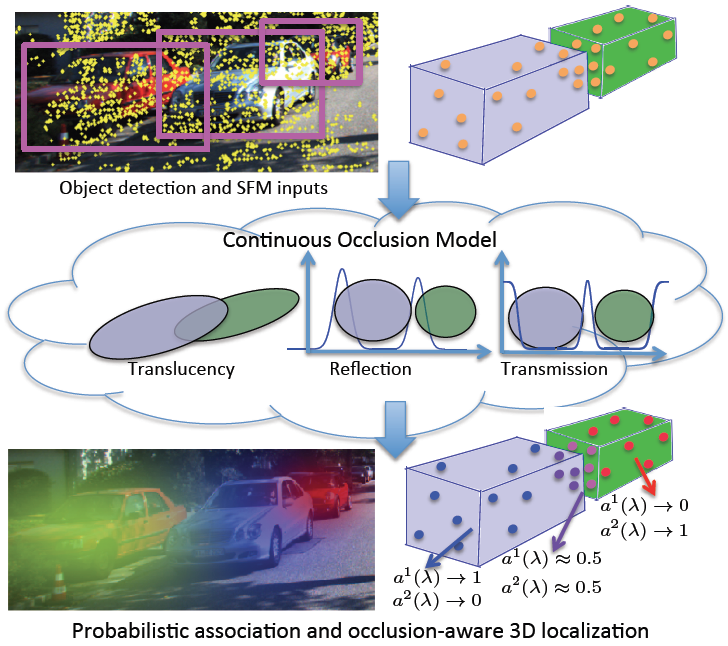
\includegraphics[width=0.7\linewidth]{graphics/figure1.png}
\end{center}




        \end{figure}
      \end{block}

      \begin{block}{Continuous Occlusion Model}
        \begin{align}
          f^i_{\text{occ}}(\bx) = \cL(\bx; \bp_i, \bSigma_i),
        \end{align}
        \begin{align}
          P^{ij}_{\textit{observation}} = P^{ij}_{\textit{reflection}}P^{j}_{\textit{transmission}}.
          \label{eq:imgform}
        \end{align}
        \begin{align}
          \Prefl = \frac{1}{Z}(\max \{0, \nabla {f^i_{occ}}(\bx_j)^\top \ray \})^2.
          \label{eq:evalPrefl}
        \end{align}

        \begin{align}
          P^j_{\textit{transmission}}(\lambda) &= \prod_{c}^{\lambda} (1 - \occft{\lambda \ray})^{d\lambda}\\
          &\approx \prod_i (1 - \cL_u (\bu; \bmu_i, \bGamma_i) \cL_{\lambda}(\lambda; \meandepth{i})).
          \label{eq:ptrans-integral}
        \end{align}

        % \begin{figure}
        %   \usetikzlibrary{calc}
        %   \centering
        %   \begin{tikzpicture}
        %          \path [fill=blue!20,draw] (0,0) ellipse (1.2 and 0.7);
     \path [fill=green!20,draw] (3,0) ellipse (1.2 and 0.7);
     \coordinate (o) at (-2,-1);
     \draw(o) edge [->,very thick] node (xa) {} +(6, 0);
     \node at ($(xa) + (0, -0.2)$) {Depth from camera($\lambda$)};
     \draw(o) edge [->,very thick] node (ya) {} +(0, 2);
     \node [rotate=90]at ($(ya) + (-0.2, 0)$) {Probability};
    \draw [thick,blue]plot [smooth] coordinates {($(o)+(0,0.2)$) ($(o)+(0.2,0.2)$) ($(o) + (0.8, 1.8)$) ($(o)+(1.6,0.2)$) ($(o)+(3.2,0.2)$) 
      %($(o)+(3.8,1.8)$)  % Transmission prob corresponds to particular object
    ($(o)+(4.4,0.2)$) ($(o)+(6.4,0.2)$) };
    \draw [thick,red] plot [smooth] coordinates {($(o)+(0,1.8)$) ($(o)+(0.2,1.8)$) ($(o) + (0.8, 1.7)$) ($(o)+(1.4,0.2)$) ($(o)+(2.6,0.2)$) ($(o)+(3.2,1.8)$) ($(o)+(3.8,1.8)$) ($(o)+(4.4,0.2)$) ($(o)+(5.6,0.2)$) ($(o)+(6.1,1.8)$) };
   \draw [thick, blue] ($(o) + (0,-0.5)$) -- +(1,0) +(2,0) node {$P_{\text{reflection}}$};
   \draw [thick, red] ($(o) + (3,-0.5)$) -- +(1,0) +(2,0) node {$P_{\text{transmission}}$};

        %   \end{tikzpicture}
        %   \vspace{-0.3cm}
        %   \caption{\small We represent objects as translucent ellipsoids, which leads to the formulation of transmission and reflection probabilities. This figure shows the reflection probability for the first object (in violet), which has high values around the camera-facing side of the object. Also, note that the transmission probability is inversely proportional to occupancy.}
        %   \label{fig:reflectiontransimission}
        %   \vspace{-0.3cm}
        % \end{figure}
        \begin{figure}
          \centering
          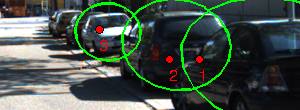
\includegraphics[width=0.9\columnwidth]{results/plotPtransmission_exact_vs_approx_pt_vis-small.png}\\
          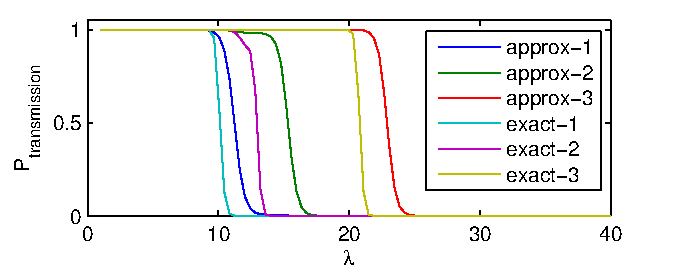
\includegraphics[trim=0.0 0 0.3in 0, clip, width=0.9\columnwidth]{results/plotPtransmission_exact_vs_approx_embedded_fonts.pdf}
          \vspace{-0.3cm}
          \caption{\small Comparisons between the approximate and exact formulations of $\Ptrans$. The drop in the approximate version is delayed because we assume drop at the object center rather than the camera-facing face of the object.}
          \label{fig:compare:exact:approx:ptrans}
          \vspace{-0.3cm}
        \end{figure}
      \end{block}

    \end{column}
    \begin{column}{\sepwid}\end{column}			% empty spacer column
    \begin{column}{2.0\onecolwid}
      \begin{block}{Results}
        \vspace*{-\baselineskip}
        \begin{columns}[t]
          \column{1.000\onecolwid}
          \begin{table}
            \begin{tabular}{lrrrr}
              \toprule
              Point tracks & Ours & BBox & BM & RAS\\
              \midrule
              Dynamic \& occluded         & \textbf{13.2} & 21.3 & 30.9 & 30.1 \\
              Occluded		              & \textbf{15.7} & 19.8 & 39.5 & 37.8 \\
              Dynamic		              & \textbf{6.6} & 11.4 & 15.3 & 17.7 \\
              All		                  & \textbf{8.6} & 12.6 & 21.9 & 21.5 \\
              \bottomrule
            \end{tabular}
            \caption{\small Mean association errors on different sets of input point tracks over all sequences. Errors are in terms of average fractions of foreground points incorrectly associated to objects per sequence.}
            \label{tab:meanAssoc}
          \end{table}
          \column{1.000\onecolwid}
          \begin{table}
            \begin{tabular}{lrr}
              \toprule
              Method & t & dim \\
              \midrule
              Point cloud fitting
              & 6.87 & 4.02\\
              Initialization by~\cite{Song_Chandraker_2014}
              & 5.61 & 3.23\\
              $\EnergyTrackNoOcc + \EnergyBBoxNoOcc +\EnergySize+\EnergyDyn$ 
              & 3.95  & 1.72\\        
              $\EnergyTrackNoOcc + \EnergyBBox +\EnergySize+\EnergyDyn$        
              & 4.81  & 2.16\\        
              $\EnergyTrack + \EnergyBBoxNoOcc +\EnergySize+\EnergyDyn$      
              & 4.05  & {\bf 1.59}\\        
              $\EnergyTrack + \EnergyBBox +\EnergySize+\EnergyDyn$             
              & {\bf 3.24}  & 2.16\\
              \bottomrule
            \end{tabular}
            \caption{\small Localization experiment results with different combinations of energies. We report translation error (t) and dimension error (dim) in meters per car. Yaw angles for static objects are not optimized by our model. These experiments use the set of occluded tracks to demonstrate the effect of our modeling.}
            \label{tab:localizationExperiment}
          \end{table}
        \end{columns}
      \end{block}

      \begin{block}{Association error}
        \begin{figure}[!!t]
          \centering
          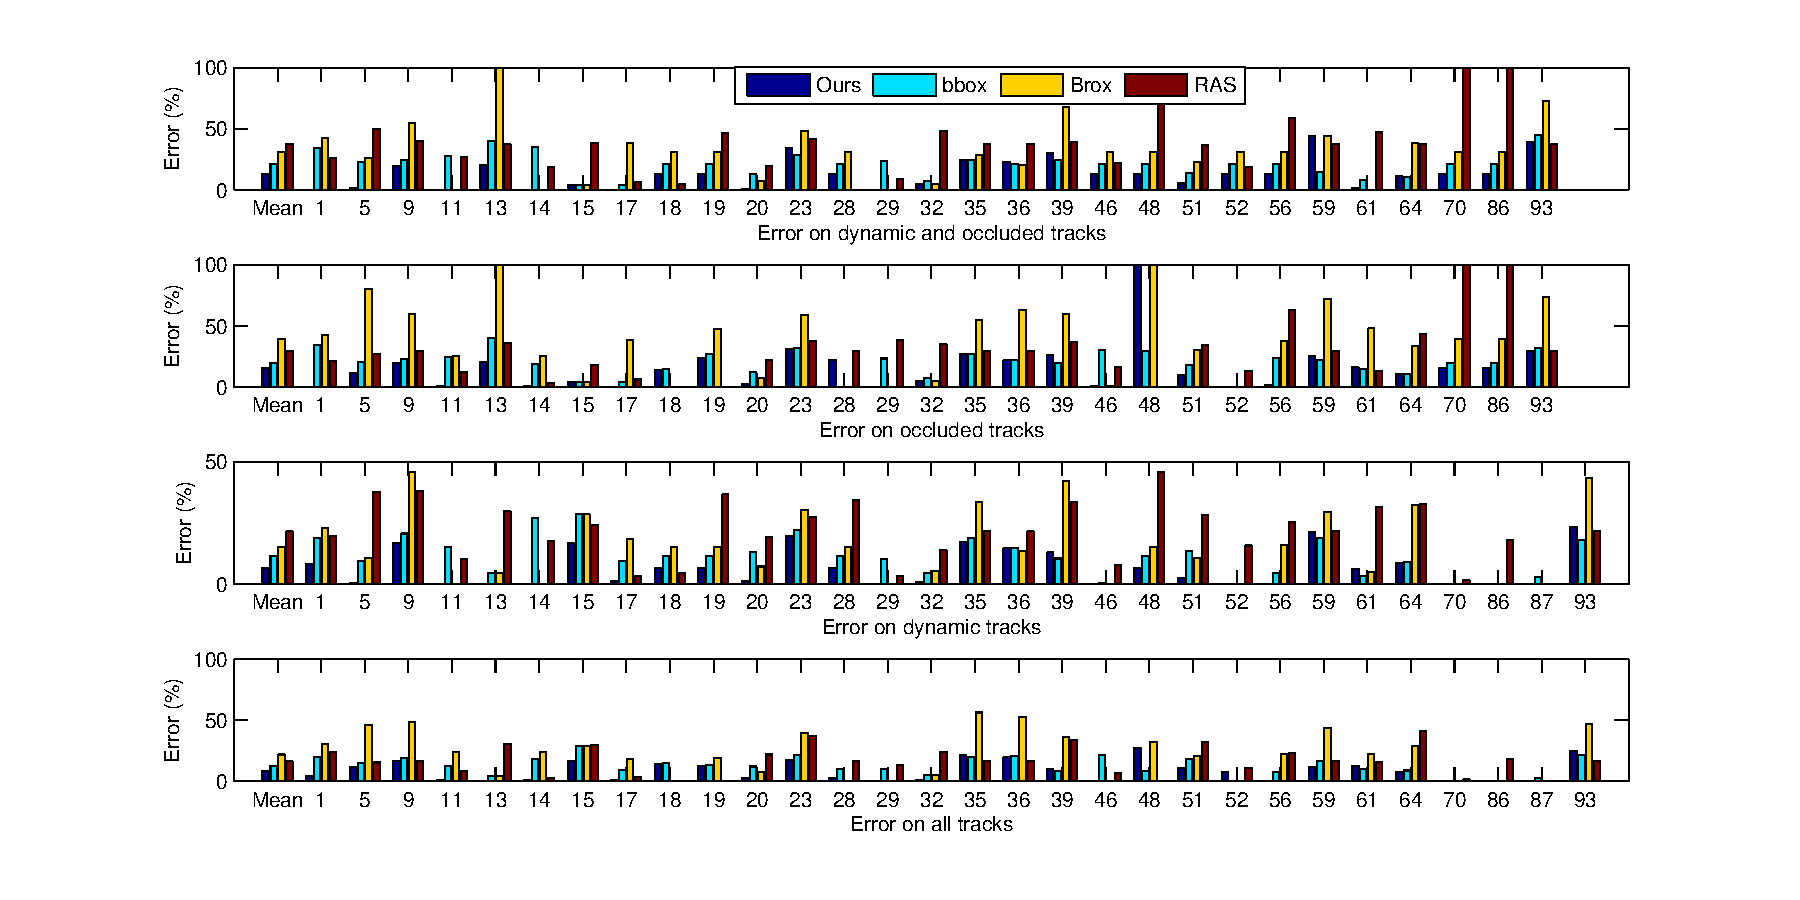
\includegraphics[trim=1.0in 0.4in 1.0in 0.2in, clip, width=0.9\textwidth]{results/plotErrorBarEvalAssocCoeffAllSequence.pdf}
          \vspace{-0.3cm}
          \caption{\small Association errors on different sets of input point tracks. Numbers on the x-axis represent sequence numbers in the KITTI raw dataset. Errors are in terms of average fractions of foreground points incorrectly associated to objects per sequence.}
          \vspace{-0.3cm}
          \label{fig:assoc-occ-results}
        \end{figure}
        \newlength{\tblimgwidth}
        \setlength{\tblimgwidth}{0.080\textwidth}
                \begin{figure}[!!t]
          \centering
          \begin{tabular}{cc@{}c@{\hspace{0.1cm}}c@{}c@{}}
            & Associations & Errors & Associations & Errors\\
            \rotatebox{90}{\hspace{1em} RAS}%
            & 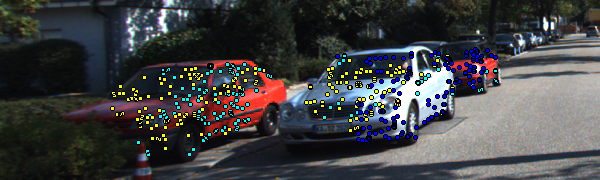
\includegraphics[height=\tblimgwidth]{results/0009_0000000060_point_assign_RAS-small.png}%
            & 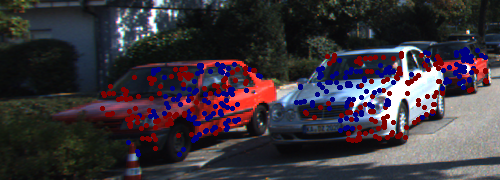
\includegraphics[height=\tblimgwidth]{results/0009_0000000060_point_assign_RAS_correct_incorrect-small.png}%
            & 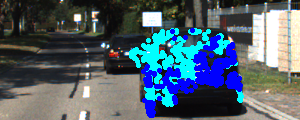
\includegraphics[height=\tblimgwidth]{results/0013_0000000060_point_assign_RAS-small.png}%
            & 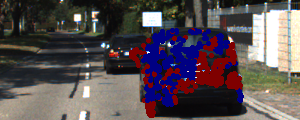
\includegraphics[height=\tblimgwidth]{results/0013_0000000060_point_assign_RAS_correct_incorrect-small.png}\\
            \rotatebox{90}{\hspace{1em} BM}%
            & 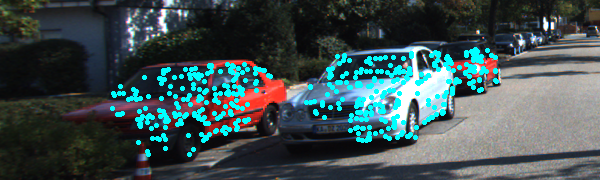
\includegraphics[height=\tblimgwidth]{results/0009_0000000060_point_assign_BroxAndMalik2010-small.png}%
            & 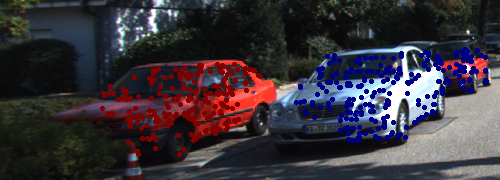
\includegraphics[height=\tblimgwidth]{results/0009_0000000060_point_assign_BroxAndMalik2010_correct_incorrect-small.png}%
            & 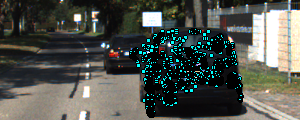
\includegraphics[height=\tblimgwidth]{results/0013_0000000060_point_assign_BroxAndMalik2010-small.png}%
            & 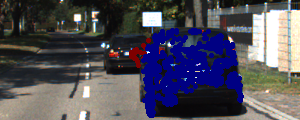
\includegraphics[height=\tblimgwidth]{results/0013_0000000060_point_assign_BroxAndMalik2010_correct_incorrect-small.png}\\    
            \rotatebox{90}{\hspace{1em} BBox}%
            & 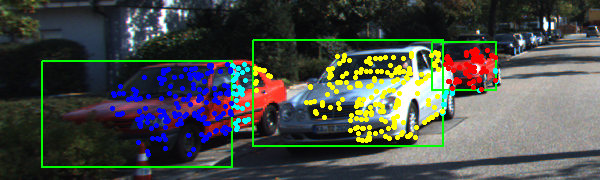
\includegraphics[height=\tblimgwidth]{results/0009_0000000060_point_assign_bbox2D_model-small.png}%
            & 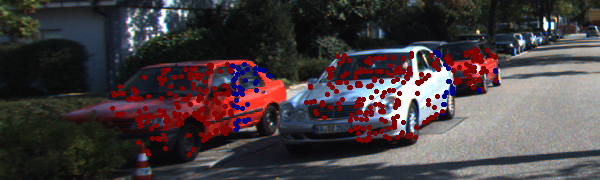
\includegraphics[height=\tblimgwidth]{results/0009_0000000060_point_assign_bbox2D_model_correct_incorrect-small.png}%
            & 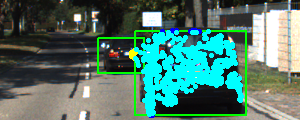
\includegraphics[height=\tblimgwidth]{results/0013_0000000060_point_assign_bbox2D_model-small.png}%
            & 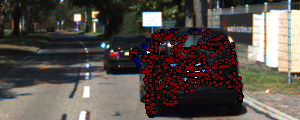
\includegraphics[height=\tblimgwidth]{results/0013_0000000060_point_assign_bbox2D_model_correct_incorrect-small.png}\\
            \rotatebox{90}{\hspace{1em} Ours}%
            & 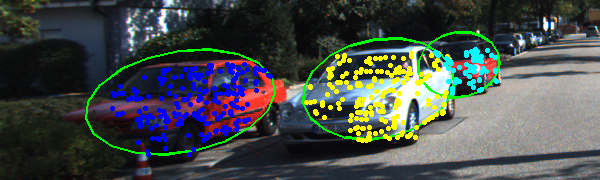
\includegraphics[height=\tblimgwidth]{results/0009_0000000060_point_assign_contPtTracks-small.png}%
            & 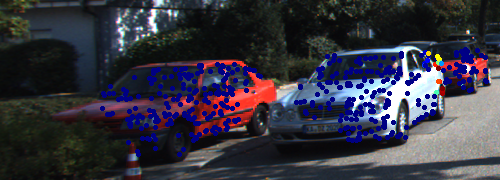
\includegraphics[height=\tblimgwidth]{results/0009_0000000060_point_assign_contPtTracks_correct_incorrect-small.png}%
            & 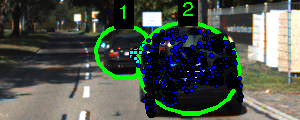
\includegraphics[height=\tblimgwidth]{results/0013_0000000060_point_assign_contPtTracks-small.png}%
            & 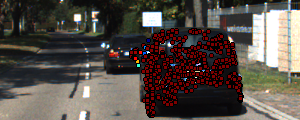
\includegraphics[height=\tblimgwidth]{results/0013_0000000060_point_assign_contPtTracks_correct_incorrect-small.png}
          \end{tabular}
          \vspace{-0.3cm}
          \caption{\small Qualitative results of the association experiment. The ``Associations" columns
            show the point track assignments to appropriate objects. Each color represents
            a different object to which point tracks can be associated to. The ``Errors" columns show the
            probabilistic errors in association: low error points are in blue while high error points are in red.
            Note that our method changes smoothly at the object boundaries with
          intermediate probabilities, while the baseline method has merely 0 and 1 errors.}
          \label{fig:qualitative}
          \vspace{-0.3cm}
        \end{figure}

      \end{block}
    \end{column}
    \begin{column}{\sepwid}\end{column}			% empty spacer column
    \begin{column}{\onecolwid}
      \begin{block}{Object Point Association}
        \begin{align}
          \assocP = \Prefl\Ptrans,
          \label{eq:defineassocP}
        \end{align}
        \begin{align}
          P^{ij}_{\text{assoc}} = \frac{1}{Z''}\int_0^{\infty} \assocP \exp(-\Ereproj(\lambda))d\lambda,
          \label{eq:prob-assoc}
        \end{align}
      \end{block}
      \vspace{0.5in}
      \begin{block}{3D Object Localization}
        \begin{figure}
          \centering
          \usetikzlibrary{trees,shadows}
\begin{tikzpicture}[grow cyclic, line width=1.2pt,
    variablenode/.style={circle,circular drop shadow,draw=red,fill=white,thick,minimum width=0.5cm},
   bboxfactor/.style={rectangle,drop shadow,draw=green,fill=green,thick,minimum width=0.2cm},
    collfactor/.style={rectangle,drop shadow,draw=blue,fill=blue,thick,minimum width=0.2cm},
    trackfactor/.style={rectangle,drop shadow,draw=red,fill=red,thick,minimum width=0.2cm},
  obs/.style={fill=gray!30,draw=black},
  prevf/.style={draw=green!20,text=gray},
  prevobsv/.style={draw=gray!10,fill=gray!1,text=gray},
  prevv/.style={draw=red!20,text=gray}
]
  \path[use as bounding box,clip] (-2.5, -5.5) rectangle (5.5,0.5);
  \draw (-2.5,-2.65) rectangle +(0.5,0.3);
  \draw (-2.0,-2.35) -- ++(0.15, 0.15) -- ++(0, -0.6) -- (-2.0, -2.65);
\path
     (0, 0)  node [variablenode] (x6) {6}
++(0, -1.5) node [variablenode] (x2) {2}
++(2.5, 0)  node [variablenode] (x5) {5}
+ (0, 1.5)  node [variablenode,obs] (u) {}
+(.2,1.0)  node {$u$}
+ (.5, -2)   node [variablenode] (x3) {3}
+ (2.3, -3.5)   node [variablenode] (x4) {4}
+(2.5, 0)  node [variablenode] (x1) {1}
;

% Factors between nodes 6 and 2
\draw (x6) edge [bend right=35] node [bboxfactor] (f26) {} (x2);
\path (f26) +(-0.75,0) node [variablenode,obs] (d6) {} 
                        +(-.7,-.6)  node {$d^6$};
\draw (f26) edge (d6);
\draw (x6) edge [bend left=35] node [trackfactor] (ft26) {} (x2);
\draw (ft26) edge [bend left=10] (u);
\draw (x6) edge node [collfactor] {} (x2);

% Factors for node 2
\path (x2) +(0,-1.25) node [variablenode,obs] (d2) {} 
                        +(-.6,-1.3)  node {$d^2$};
\draw (x2) edge node [bboxfactor] {} (d2);

% Factors between nodes 2 and 5
\draw (x2) edge [bend right] node [bboxfactor] (f25) {} (x5);
\draw (x2) edge [bend left] node [trackfactor] (ft25) {} (x5);
\draw (x2) edge [] node [collfactor] {} (x5);
\draw (ft25) edge (u);
\path (x5) ++(-1.25,-1.25) node [variablenode,obs] (d5) {} 
                        +(.6,0)  node {$d^5$};
\draw (f25) edge (d5);

% Factors between nodes 5 and 1
\draw (x5) edge [bend right] node [bboxfactor] (f51) {} (x1);
\draw (x5) edge [bend left] node [trackfactor] (ft51) {} (x1);
\draw (x5) edge [] node [collfactor] {} (x1);
\draw (ft51) edge [bend right] (u);
\path (x1) ++(-1.25,-1.25) node [variablenode,obs] (d1) {} 
                        +(-.5,0.2)  node {$d^1$};
\draw (f51) edge (d1);

% Factors for node 3
\path (x3) ++(0,-1.25) node [variablenode,obs] (d3) {} 
                        +(.6,0)  node {$d^3$};
\draw (x3) edge node [bboxfactor] {} (d3);

% Factors for node 4
\path (x4) ++(0,1.25) node [variablenode,obs] (d4) {} 
                        +(.6,0)  node {$d^4$};
\draw (x4) edge node [bboxfactor] {} (d4);

% Legend
\path (-1.75,-4.0) node (l1s) {} (-0, -4.0) node [anchor=west] (l1e) {$\Energy{bbox}$};
\draw (l1s) edge node [bboxfactor] {} (l1e);
\path (-1.75,-4.5) node (l2s) {} (0, -4.5) node [anchor=west] (l2e) {$\EnergyCol$};
\draw (l2s) edge node [collfactor] {} (l2e);
\path (-1.75,-5.0) node (l3s) {} (0, -5.0) node [anchor=west] (l3e) {$\Energy{point}$};
\draw (l3s) edge node [trackfactor] {} (l3e);

\end{tikzpicture}
%
          \caption{Graphical model showing the factor nodes among different
            cars in the same frame. We assume occlusion relationships between
            different cars are known and hence the occlusion modeling can be done
            locally. In this example, the occlusion relationship affects the
            following pair of cars 6-2, 2-5, 5-1. Cars 3 and 4 are not occluded
            and hence affected by only unary terms within the frame. We also avoid 
            collision modeling between unoccluded cars to encourage sparsity.
          }
          \label{fig:graphmodel}
        \end{figure}
        \begin{multline*}
          -\log{P(\{ \bp^i(t) , \bomega^i(t) , \bB^i(t) \} | \{\bu_j(t)\} , \{\bb{i}\} )} = \\
          -\tilde{Z} 
          + \sum_{t=s_i}^{e_i} \lambda_{\text{track}}\EnergyTrack
          + \\ 
          \sum_{t=s_i}^{e_i} \sum_{i=1}^N  
          \left(
            \lambda_{\text{detect}}\EnergyBBox
            + \lambda_{\text{dyn}}\EnergyDyn    
            + \lambda_{\text{size}}\EnergySize
          \right)
          \enspace,
        \end{multline*}
        \begin{equation}
          \Ereproj(\lambda) = \left\|\trackpj{t} - \projectionOf{\invProjectionOftm{\trackpj{t-1}, \lambda}}\right\|^2.
          \label{eq:reprojerror}
        \end{equation}
        % \begin{figure}
        %   \centering
        %   \newcommand{\imagewidth}{\onecolwid}
        %   ../../CVPR/Source/scenelayoutoverlayCity0961.tex
        %   \caption{A sample road scene with the unknowns of each car modeled as random variables. 
        %   The relating energies are shown in Figure~\ref{fig:graphmodel}}
        % \end{figure}

      \end{block}
      \vspace{0.5in}
      \begin{block}{Conclusions and Future work}
        \begin{itemize}
          \item Presented physically interpretable unified occlusion modeling
          \item The model generalizes to different applications: point association and 3D localization
          \item Challenges include the slow inference on 3D localization
        \end{itemize}
      \end{block}
      \vspace{0.5in}
      \begin{block}{Acknowledgements}
        This work was part of V.~Dhiman's internship at NEC Labs America, in Cupertino. V.~Dhiman and J.~J.~Corso were also supported by NSF NRI IIS 1522904.
      \end{block}
      \begin{block}{References}
        \bibliography{poster}
        \bibliographystyle{ieee}
      \end{block}
    \end{column}
  \end{columns}
\end{frame}

\end{document}
